\documentclass[11pt]{article}
\usepackage[utf8]{inputenc}
\usepackage{fancyhdr}
\usepackage[english]{babel}
\usepackage{graphicx}
\usepackage{array}
\usepackage{amsmath}
\usepackage{amssymb}
\usepackage{mathtools}
\usepackage{algorithmicx}
\usepackage{algpseudocode}
\renewcommand{\baselinestretch}{1.0}
\usepackage[letterpaper, margin=0.75in]{geometry}
\DeclarePairedDelimiter{\ceil}{\lceil}{\rceil}
\pagestyle{fancy}
\lhead{}
\rhead{Yu Mi, yxm319. Algorithm HW3}
\begin{document}
	\title{Homework3 for EECS 340}
	\author{Yu Mi,yxm319}
	\maketitle
\section{Sorting Leftover Elements}
\noindent \emph{Question}: Suppose that you are given an array consisting of $n$ sorted elements followed by $f(n)$ elements in an arbitrary order, where $f(n)\in O(n^{1-\epsilon})$ for some $\epsilon \in(0,1)$. Describe a method to sort the array in $O(n)$ time.

\noindent \emph{Answer}: This question describes a scenario similar to the intermediate steps of a merge sort, so that we need to solve this problem similar to the approach of a merge sort. First, we need to sort the leftover elements with merge sort, which takes $O(n^{1-\epsilon}\cdot \log n^{1-\epsilon})$ time. After that, we will need to merge the two sequence (original sorted one and the left over part) into a whole sorted sequence, which takes $O(n)$ time. To show that $O(n^{1-\epsilon}\cdot \log n^{1-\epsilon})$ takes less time than $O(n)$, we assign $g(n)=n^{1-\epsilon}\cdot \log n^{1-\epsilon}$, $h(n) = n$. Thus we have:
\begin{equation*}
	\lim_{n\to\infty} \frac{g(n)}{h(n)} = \lim_{n\to\infty}\frac{(1-\epsilon)\cdot n^{1-\epsilon}\cdot\ln n}{n\cdot \ln 2}= \lim_{n\to\infty} \frac{(1-\epsilon)^2}{\ln 2}\cdot(n^{-\epsilon}\cdot \ln n + n^{-\epsilon}) =\lim_{n\to\infty} \frac{(1-\epsilon)^2}{\ln 2} \cdot \frac{\ln n +1}{n^{\epsilon}} =\lim_{n\to\infty} \frac{(1-\epsilon)^2}{\ln 2} \cdot \frac{1}{\epsilon n^{\epsilon}}
\end{equation*}

L'Hospital's rule is used in the second and forth step. The equation above will approach $0$ when $n\to \infty$, so that $O(n^{1-\epsilon}\cdot \log n^{1-\epsilon})$ takes less time than $O(n)$, we can conclude that $O(n^{1-\epsilon}\cdot \log n^{1-\epsilon}) + O(n)$ is $O(n)$. 
\section{Theory: Sorting Algorithm Run-times}
\subsection{Give a tight asymptotic bound on $f(n)$}
\noindent \emph{Answer}: Since the total amount of permutation od $n$ elements is $n!$, and binary encoding will use $\log (n!)$ bits to encode such permutations, our tight asymptotic bound should be 
\begin{equation*}
\log(n!)=\sum_{i=1}^{n} \log i
\end{equation*}
Such time bound make sense because it is always smaller than $n\log n$, which is the time of fastest sorting algorithm (at least I know).
\subsection{Why doesn't the derived lower bound, from the previous part hold for non-comparison-based sorting algorithms like radix sort.}
\noindent \emph{Answer}: Since non-comparison-based is not based on comparisons to make a sort, they cannot be viewed as a comparison-based approach where each comparison can be treated as searching for a bit in the permutation. The lower bound derived above only stands for the comparison based sorting algorithm where we use each comparison to compose a 'bit' for the ultimate answer.
\section{Post Office Placement}
\noindent \emph{Question}: Suppose you are the postmaster in charge of putting a new post office in a small town, where all the houses are along one street, where the new post office should go as well. Let us view this street as a line and the houses on it as a set of real numbers, $\{x_1, x_2, . . . , x_n\}$, corresponding to points on this line. To make everyone in town as happy as possible, the location, p, for the new post office should minimize the sum,
\begin{equation*}
	\sum_{i=1}^{n} |p-x_i|.
\end{equation*}
Describe an efficient algorithm for finding the optimal location for the new post office, show that your algorithm is correct, and analyze its running time.

\noindent \emph{Answer}: To solve this problem, we can first consider two houses, where we can simply conclude that the best post office position for this two houses is the middle of their address. The we can extend this conclusion to a three house scenario, where the middle point calculated can be seen as having a weight of $2$ and the third house have a weight of $1$, then we can conclude that the weighted average point is the optimal position for the new post office. Another notable fact is that we can calculate the average point recursively, which will achieve a time complexity of $O(\log n)$. The algorithm can be shown as follow:
\begin{algorithmic}
	\State \textbf{Algorithm} FindPostOffice($S,n$)
	\State \textbf{Data}: An address sequence $S$, and its length $n$
	\State \textbf{Result}: The best position for a new post office.
	\If{$n==1$}
		\State \Return $S[n]$
	\EndIf
	\If{$n==2$}
		\State \Return $(S[0]+S[1])/2$
	\EndIf
	\If{$n\%2==0$}
		\State \Return $FindPostOffice(S,n/2)+FindPostOffice(S+n/2,n/2)$
	\Else
		\State $Middle\gets (n-1)/2$
		\State $LeftPart \gets (Middle/n)\times FindPostOffice(S,Middle)$
		\State $RightPart \gets (n-Middle/n)\times FindPostOffice(S+Middle,n-Middle)$
		\State \Return $LeftPart+RightPart$
	\EndIf
\end{algorithmic}
\section{Sorting Sequences}
\noindent \emph{Question}: Suppose we are given a sequence $S$ of $n$ elements, each of which is an integer in the range $[0,n^2-1]$. Describe a simple method for sorting $S$ in $O(n)$ time.

\noindent \emph{Hint}: Think of alternate ways of viewing the elements.
\noindent \emph{Answer}: The approach is based on Radix sort:
\begin{algorithmic}
	\State \textbf{Algorithm} Radix-sort($S,n$)
	\State \textbf{Data}: A unsorted sequence $S$, and its length $n$
	\State \textbf{Result}: The sorted sequence $S'$
	\State $buckets \gets n $ lists
	\For{$i \gets 0$ to $n$}
		\State $digit \gets $\textbf{int}$((S[n])/n)$
		\State $buckets[digit]$.append($S[n]$)
	\EndFor
	\For{$i \gets 0$ to $n$}
		\State $result\gets n$ lists
		\For{$j\gets 0$ to $length(buckets[i])$}
			\State $result[buckets[i][j]\%n].append(buckets[i][j])$
		\EndFor
		\State $bucket\gets$ empty list
		\For{$j\gets 0$ to $n$}
			\State $bucket.append(result[j])$
		\EndFor
		\State $buckets[i]\gets bucket$
	\EndFor
	\State $result \gets$ empty list
	\For {$i \gets 0$ to $n$}
		\For {$number$ in $bucket[i]$}
			\State $result.append(number)$
		\EndFor
	\EndFor
\end{algorithmic}
\section{Median From Two Lists}
\noindent \emph{Question}: Suppose you are given two sorted lists, $A$ and $B$, of $n$ elements each all of which are distinct. Describe a method that runs in $O(\log n)$ time for finding the median in the set defined by the union of $A$ and $B$. Note that merging or concatenating the arrays would take $O(n)$ time.

\noindent \emph{Answer}: The approach is based on recursive and dividing:
\begin{algorithmic}
	\State \textbf{Algorithm} GetMedian($A,B,n$)
	\State \textbf{Data}: Two sorted list $A$ and $B$, and their length are both $n$
	\State \textbf{Result}: The median of the union of $A$ and $B$.
	\If{$n == 1$}
		\State \Return $(A[0]+B[0])/2$
	\EndIf
	\If{$n\%2==0$} \Comment Get the median of $A$ and $B$
		\State $m1\gets (A[n/2]+A[n/2-1])/2$
		\State $m2\gets (B[n/2]+B[n/2-1])/2$
	\Else
		\State $m1\gets A[n/2]$
		\State $m2\gets B[n/2]$
	\EndIf
	
	\If{$m1==m2$} \Comment If the median are equal, return either $m1$ or $m2$
		\State \Return m1
	\EndIf
	
	\If($m1 < m2$)
		\If{$n\%2==0$}
			\State \Return $GetMedian(A+n/2-1,B,n-n/2+1)$ \Comment The add operation to a list name is same as C language which means to shift the pointer to the next $n/2-1$ address.
		\Else
			\State \Return $GetMedian(A+n/2,B,n-n/2)$
		\EndIf
	\Else
		\If{$n\%2==0$}
			\State \Return $GetMedian(B+n/2-1,A,n-n/2+1)$
		\Else
			\State \Return $GetMedian(B+n/2,A,n-n/2)$
		\EndIf
	\EndIf
\end{algorithmic}

	To achieve the $O(\log n)$ time complexity, we need to try divide and recursively solve the problem. First we need to calculate the medians of $A$ and $B$, and then compare them. If $m1$ and $m2$ are equal, we are simply done. Otherwise, if $m1<m2$, we can conclude that the median is in the two list, one is from $m1$ to the last element of $A$ and the other one is from the first element of $B$ to $m2$. It is the similar process when $m1>m2$. When the two arrays have a size of $1$, we can simply calculate their average as the result.
\section{Warm-up: Graphs}
\subsection{R-7.1}
\noindent \emph{Question}: Suppose we have a social network with members $A,B,C,D,E,F,$ and $G$, and the set of friendship ties,
\begin{equation*}
	\{(A,B),(B,C),(C,A),(D,E),(F,G)\}.
\end{equation*}
Where are the connected components?

\noindent \emph{Answer}: The connection relationship can be represented by the Fig.\ref{fig:fig1}.
	\begin{figure}[h]
		\centering
		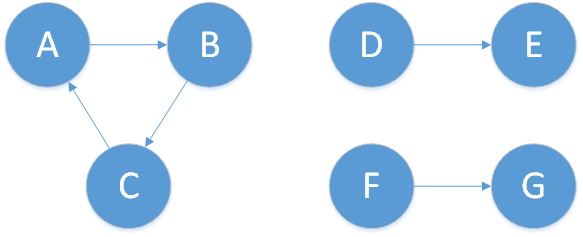
\includegraphics[width=0.4\textwidth]{Figure/Fig1.png}
		\caption{Relation graph}
		\label{fig:fig1}
	\end{figure}

From the figure we can conclude that the connect components are $(A,B,C)$, $(D,E)$ and $(F,G)$.
\subsection{R-13.2}
\noindent \emph{Question}: Let $G$ be a simple connected graph with $n$ vertices and $m$ edges. Explain why $O(\log m)$ is $O(\log n)$.

\noindent \emph{Answer}: When we have $m$ vertices, the maximum number of edges could be $m<n(n-1)<n^2$, which means $O(\log m)<O(\log n^2)= O(2\log n)=O(\log n)$. To sum up, $O(\log m)$ is $O(\log n)$.
\subsection{Given the graph}
\subsubsection{Draw the graph where all nodes are annotated with the order that they are visited in a \textbf{depth-first} search from A.}
\noindent \emph{Answer}: The result is shown in Fig. \ref{fig:fig2}.
	\begin{figure}[h]
		\centering
		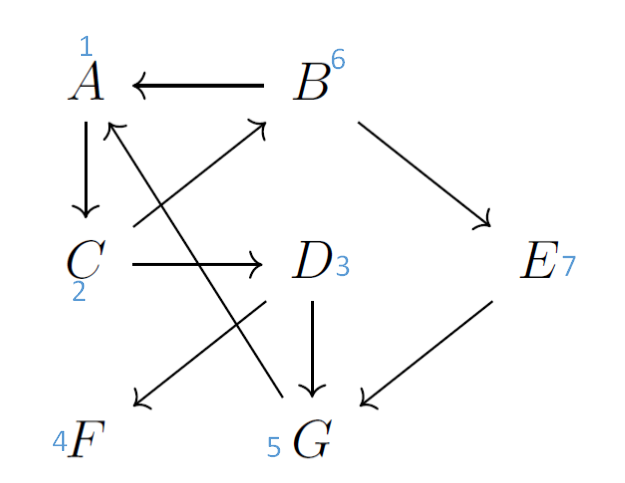
\includegraphics[width=0.4\textwidth]{Figure/Fig3.png}
		\caption{Annotated graph}
		\label{fig:fig2}
	\end{figure}
\subsubsection{Draw a representation of the tree generated by the DFS annotated over the previous part.}
\noindent \emph{Answer}: The result is shown in Fig. \ref{fig:fig3}.
	\begin{figure}[h]
		\centering
		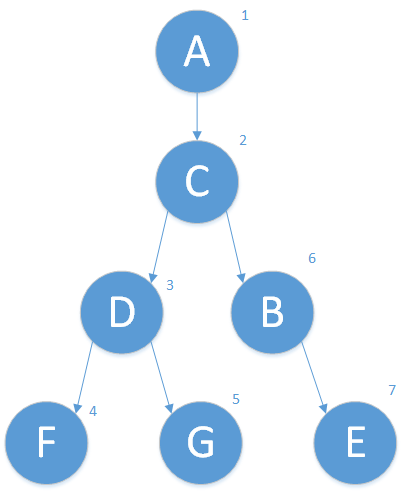
\includegraphics[width=0.4\textwidth]{Figure/Fig2.png}
		\caption{Tree graph}
		\label{fig:fig3}
	\end{figure}
\section{Application: Chess}
\noindent \emph{Answer}:
\section{Application: A World of Voxels}
\noindent \emph{Answer}:
\section{Practice: Topological Sorting}
\noindent \emph{Answer}:
\section{EECS 454 only}
\subsection{C-17.4}
\noindent \emph{Question}: Consider the problem \textbf{DNF-SAT}, which takes a Boolean formula $S$ in disjunctive normal form (DNF) as input and asks whether $S$ is satisfiable. Describe a deterministic polynomial-time algorithm for \textbf{DNF-SAT}.
\subsection{C-17.5}
\noindent \emph{Question}: Consider the problem \textbf{DNF-DISSAT}, which takes a Boolean formula S in disjunctive normal form (\textbf{DNF}) as input and asks whether S is dissatisfiable, that is, there is an assignment of Boolean values to the variables of S so that it evaluates to 0. Show that \textbf{DNF-DISSAT} is \emph{NP}-complete.
\end{document}